% Appendix 3: Quantitative Relationship Between Linear and Perceptual Perspective
% Source pages: 253–256

\chapter{Quantitative Relationship Between Linear and Perceptual Perspective}

\srcpage{253}

The equations obtained above hold for a function $P_1(l)$ of any form.  In order to pass
to a quantitative comparison of linear and perceptual perspectives, we choose this function
as follows:
\begin{equation}
  P_1(l) = 1 + \arctan l.
  \tag{3.1}
\end{equation}

\srcpage{254}

It is easy to verify that the chosen function satisfies all the conditions enumerated above:
it is continuous and monotone, $P_1(0) = 1$, $P_1(\infty) = 1 + \pi/2$, and
\[
  \left.\frac{dP_1}{dl}\right|_{l=0} = \frac{1}{1+l^2}\bigg|_{l=0} = 1.
\]
Thus the function $P_1(l) = 1 + \arctan l$ qualitatively satisfies the stated properties;
its quantitative correspondence to visual perception can be confirmed only by experiment.

Fig.\,3.1 shows the dependences $y_1 = f_1(x_1)$ and $y_2 = f_2(x_2)$.  The first is
obtained from equation~(1.4), and the second by means of equations~(2.1) and~(3.1).  If
the first dependence gives the linear-perspective image of the right edge of a road, the
second is a mixed dependence: the quantity~$y$ is taken for linear perspective and $x$~for
perceptual perspective.  Such a mixed dependence does not represent the perceptual
perspective, but it does allow one to estimate easily the effect of the size-constancy
mechanism: the values of the abscissae $x_1$ and $x_2$ corresponding to the same value
of~$y_1$ also correspond to the same value of~$l$, and consequently their ratio gives a
clear representation of the contribution of the constancy mechanism to the process of
transforming the retinal image into the perceptual one.  Also shown in Fig.\,3.1 are
experimental points, which testify to a sufficiently good quantitative agreement of the
chosen dependence $P_1(l) = 1 + \arctan l$ with the data of human visual perception.

\begin{figure}[H]
    \centering
    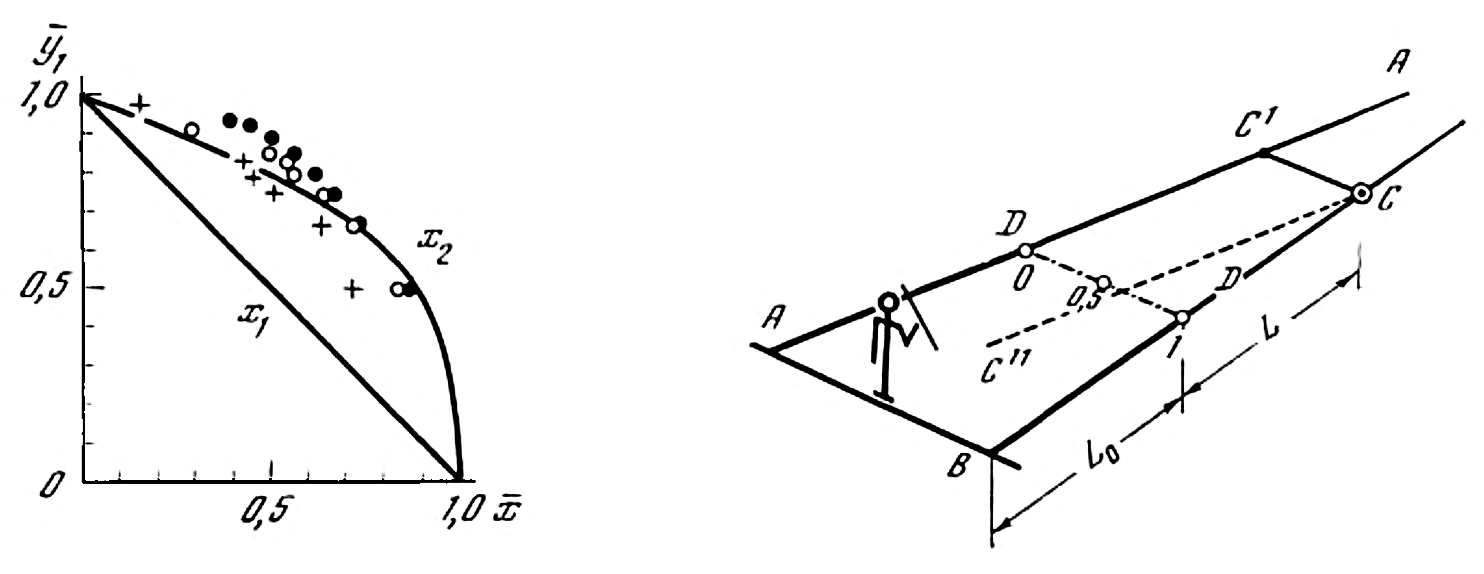
\includegraphics[width=0.95\linewidth]{figures/f3.1-f3.2.png}
\end{figure}
\figblock{3.1}{Comparison of the linear-perspective edge curve $y_1 = f_1(x_1)$ and the
  mixed perceptual curve $y_2 = f_2(x_2)$ for the right edge of a road, together with
  experimental points (filled circles: path width 1\,m; open circles: 2\,m; crosses: 5\,m).}
\figblock{3.2}{Scheme of the experiment for measuring the apparent width $x_2$ at various
  distances from the observer.  The experimenter aligns the ruler edge through object~$C$
  so that it appears parallel to the left edge $AA$ of the path; the scale $OO$ gives $x_2$
  directly.}

In order to make clear the degree of reliability of the experimental results cited, let us
describe the methodology of the experiment for measuring the quantity~$x_2$.  Since the
problem being solved is that of obtaining an image of a straight road, the experiment was
conducted in the field by measuring the apparent width of a road at various distances from
the observer.  The experimental methodology was designed so as to measure precisely the
apparent width, not the retinal image.

\srcpage{255}

Fig.\,3.2 shows the scheme of the experiment.  At a distance $l_0$ from the experimenter,
standing at the midpoint of a narrow straight path and looking along it, a line is drawn on
the surface of the path perpendicular to its axis and marked in fractions of the path's width.
Along the right edge of the path, at a previously known distance~$l$, some visible small
object~$C$ is placed.  Holding a ruler and looking with one eye, the experimenter aligns
the edge of the ruler with the object~$C$, which is at distance $l_0 + l$ from him.  The
task is that the edge of the ruler passing through~$C$ should appear parallel to the left
edge $AA$ of the path (the trace of the ruler's edge on the ground is shown by the dashed
line $CC''$).  Having achieved this, the experimenter takes a reading on the scale $OO$
along the ruler's edge and thereby determines the apparent size of the width $CC'$ in
relation to the size $OD$, taken as unity.  Obviously, the reading on the scale $OO$
directly gives the value of~$x_2$.  By moving object~$C$ (varying~$l$), one obtains the
dependence of $x_2$ on~$l$, and then via formula~(1.2) on~$y_1$.  These are precisely the
points plotted in Fig.\,3.1.\footnote{If the experimenter had measured the segment $CC'$
  by aligning the measuring device with both $C$ and $C'$ and then transferring that size
  to the segment $OD$ to assess its magnitude as a fraction of the road's width (as is
  sometimes done when learning to draw), the experimental points in Fig.\,3.1 would have
  fallen not near the curve $x_2$ but near the straight line $x_1$, i.e.\ they would have
  corresponded to linear perspective, since the alignment of points always occurs at the
  retinal level.}

The conviction that the adopted methodology makes it possible to measure the apparent
rather than the retinal image follows from the fact that the measuring device (the ruler) is
aligned with only one point~$C$ (this alignment is, of course, connected with alignment on
the retina of the eye), while instead of aligning the device with point~$C'$ to measure
segment $CC'$, a line $CC''$ parallel to $AA$ is constructed.  Since line $CC''$ is
constructed parallel to the apparent direction of $AA$ without aligning the measuring device
with any point of line $AA$, this construction takes place not at the retinal but at a higher
level of the human visual-perception system.

\srcpage{256}

The experimental points shown in Fig.\,3.1 were obtained under the following conditions:
path width 1\,m, $l_0 = 1$\,m, $l$ varied from 1 to 15\,m (marked by filled points); width
2\,m, $l_0 = 2$\,m, $l$ varied from 2 to 24\,m (marked by open circles); width 5\,m,
$l_0 = 5$\,m, $l$ varied from 5 to 180\,m (marked by crosses).  Comparison of the
experimental data and the conditionally adopted theoretical relation indicates that the latter
gives, on the whole, a qualitatively correct representation of the dependence $x_2 = f(l)$.
A noticeable departure of the experimental points from the curve, which gives values of the
function $P_1(l)$ that are too low, can be noted only for large~$l$ (values of $y_1$ close
to~1).

The comparatively good quantitative agreement of the law of variation of $x_2$ obtained
on the basis of $P_1(l) = 1 + \arctan l$ with the experimental data does not yet mean that
a general law of variation of $P_1$ with~$l$ has been found.  Nevertheless, the general
character of the variation of $x_2$ as a function of~$l$ is correctly conveyed.  In the
present book only the most general qualitative comparison of linear and perceptual
perspective is carried out, and therefore a quantitatively exact knowledge of the
dependence $P_1(l)$ is not necessary.  This is precisely what allows one to use in the
calculations the function $P_1(l)$ given by formula~(3.1).  Another consideration in favour
of formula~(3.1) is that it gives a good quantitative agreement with experiment also for
comparatively small~$l$ (in the case under consideration $l_0 = 2$\,m), and in particular
for a very close foreground, which is important in the analysis of medieval pictorial art.

Having the function $P_1(l)$ given by formula~(3.1), and using formula~(2.1) and
equation~(2.6), the perceptual image of the road can be computed.  For the adopted
function, equation~(2.6) takes the closed form
\begin{equation}
  y_2 = \int_0^l \frac{1 + \arctan(l)}{(1+l)^2} dl 
      = \frac{1}{4}\ln\frac{(1+l)^2}{1+l^2}+\frac{l-1}{2(1+l)}\arctan(l)
      + \frac{l}{1+l} \, ,  
  \tag{3.2}
\end{equation}
Using this formula one can construct the perceptual image of the road (shown as the right
image in Illustration~17 of the main text).

\begin{figure}[H]
    \centering
    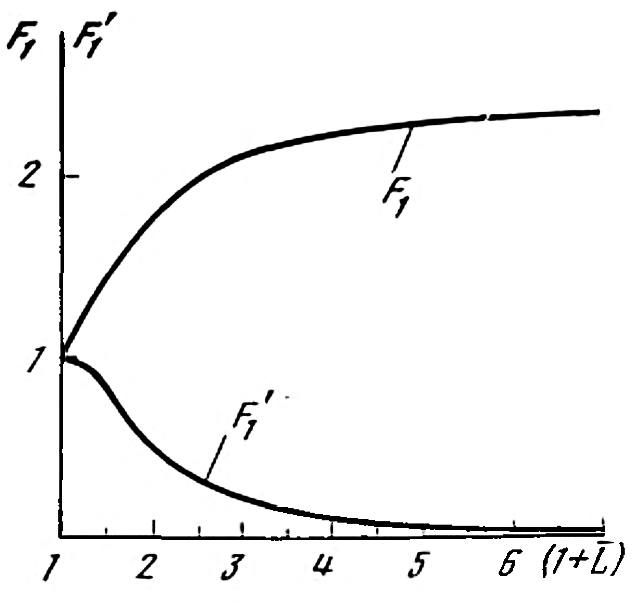
\includegraphics[width=0.4\linewidth]{figures/f3.3.png}
\end{figure}
\figblock{3.3}{Graphs of $P_1(l) = 1 + \arctan l$ and $P_1'(l) = 1/(1+l^2)$ as functions
  of the total distance $1 + l$ from the observer. $P_1$ shows the enlargement of the retinal
  image at depth $l$; $P_1'$ shows the rate of non-uniformity of that stretching.}

In conclusion it is useful to make several additional remarks.  Formula~(3.1) shows that
while for small and medium values of~$l$ the function $P_1(l)$ changes with~$l$, for
large~$l$ the value of $P_1(l)$ becomes practically constant and equal to $1 + \pi/2$.
This means that from some sufficiently large distance onward, linear and perceptual
perspectives differ only in scale: with the adopted form of $P_1(l)$, the perceptual
perspective is $1 + \pi/2 \approx 2.6$ times larger than the linear, but geometrically
similar to it.  In accordance with formula~(1.2), $y_1 \to 1$ as $l \to \infty$, while
for $P_1(l) = 1 + \arctan l$, formula~(3.2) gives

\[
  y_2 \;\xrightarrow{l\to\infty}\; 1 + \frac{\pi}{4} \approx 1.79,
\]
that is, the depth-image of space in perceptual perspective in this case is almost twice as
large as in linear perspective.

A characteristic feature of the transformation from linear to perceptual perspective (i.e.\
from the retinal image to perceptual space) is its continuity: in the course of this
transformation no gaps or discontinuities arise.  The transformation proceeds as a
``stretching''---non-uniform, to be sure, but unconditionally continuous.  Having the
specific form~(3.1) of the function $P_1(l)$, one can construct graphs relating $P_1(l)$
and $P_1'(l)$ as functions of $1 + l$ (distance from the observer); these are shown in
Fig.\,3.3.  The curve $P_1'(l)$ conveys the character of the ``stretching'' of the retinal
image: the larger this quantity, the more non-uniform the stretching of the retinal image,
which can appreciably change the geometric form of the contemplated object in the
transition from the retinal image to perceptual space.  The tendency of $P_1'$ to zero
indicates that the retinal image and the image arising in perceptual space are
geometrically approaching each other.  The curve $P_1(l)$ gives the enlargement factor of
the retinal image in the transition to perceptual space.

Taken together, both graphs show that the near zone is characterized by a significant
change by the visual-perception system in the geometric form of the object's retinal
projection without a strong change in its size, while for more distant regions of space one
observes a simple ``stretching'' of the corresponding retinal image without change of form.
This circumstance explains why, beginning from some distance, the system of linear
perspective gradually becomes natural.

In Appendix~2 the in-principle impossibility of depicting perceptual space on the picture
plane was demonstrated, yet in Illustration~17 this was done.  There is in fact no
contradiction between the statements of Appendices~2 and~3.  The point is that the image
of a road is not an image of space, because in objective space the entire road lies in the
subject plane.  Consequently, Illustration~17 gives the linear and perceptual perspectives
of the subject \emph{plane}, not of subject \emph{space}.
